\documentclass[12pt,letterpaper]{article}

\usepackage{caption} % for the figure captions
\usepackage[osf]{mathpazo} % a nicer font
% this is a package for the citation formats: found this formulation sorted natbib errors when changing packages
%from http://tex.stackexchange.com/questions/54480/package-natbib-error-bibliography-not-compatible-with-author-year-citations
\usepackage[square,sort,comma,numbers]{natbib} 
\usepackage{amsmath} % package for equations
\usepackage{url} % package for urls
\usepackage{hyperref} % for hyperlinks
\usepackage[a4paper, total={6in, 9in}]{geometry}
\hypersetup{
     colorlinks   = true,
     citecolor    = gray
}
\usepackage{graphicx} % for the figures
\usepackage{pdfpages}

\hypersetup{linkcolor=blue}

\pagenumbering{gobble}

\graphicspath{ }

\begin{document}

%title

{\Huge\textbf{\textit{Osteolepis}}\par}
\vspace{3mm}
{\large{Oss-tee-oh-leep-iss} \par} 
\vspace{5mm}
\textit{Osteolepis}

\textit{Osteolepis} is a \textbf{lobe-finned fish} from the Devonian (420 to 360 million years ago) of Scotland.  The lobe finned fishes are a group of vertebrates that includes \textbf{lungfishes, coelacanths, and tetrapods} (vertebrates that live on land).  \textit{Osteolepis} is closely related to the very earliest of this last group tetrapods and some parts of it are very similar to the very earliest amphibians.  Humans are also lobe finned fishes, as they are tetrapods, so this makes \textit{Osteolepis} your \textbf{closest relative} on this table.

\begin{figure}[h!]
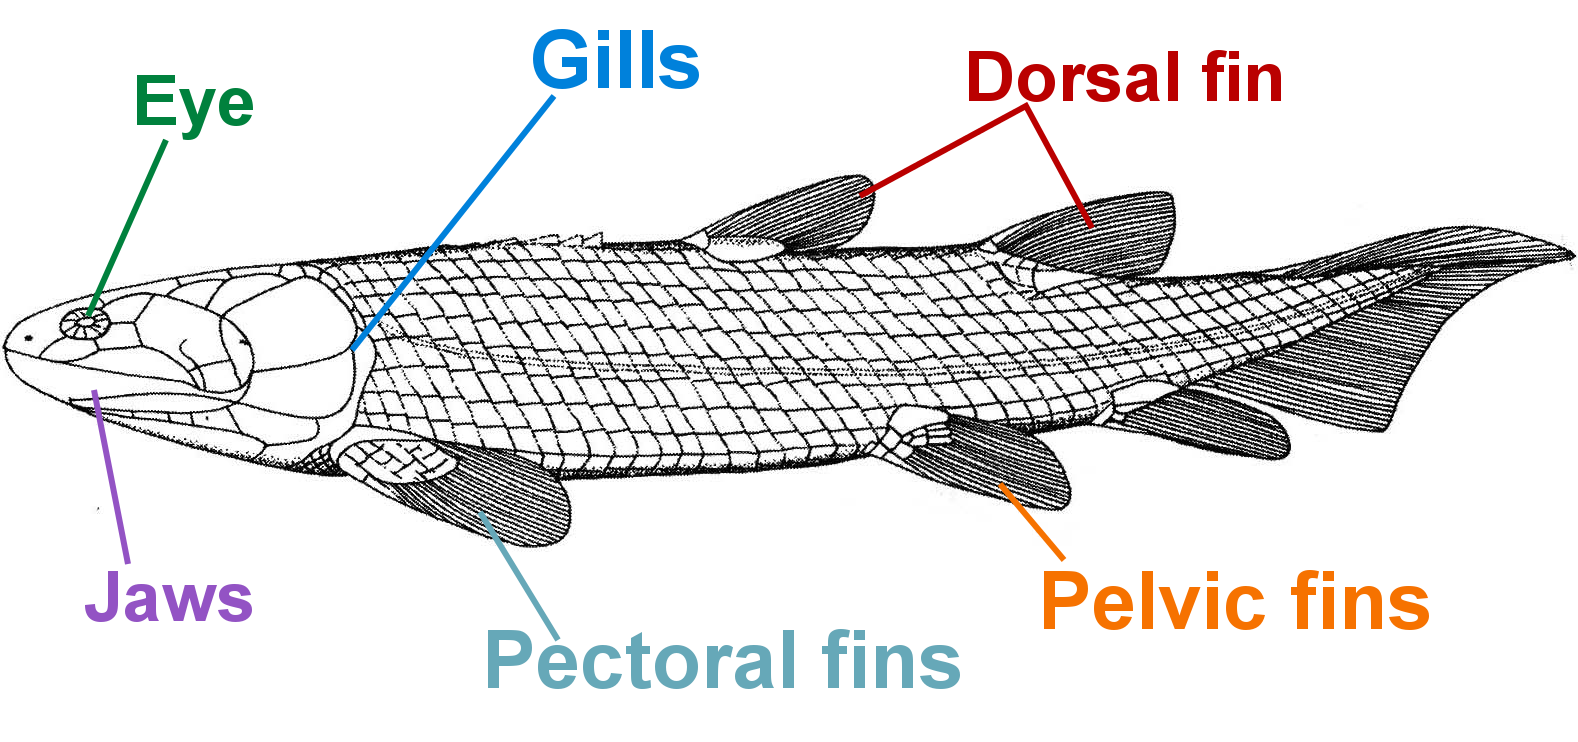
\includegraphics[scale=0.8]{Osteolepis.png}
\centering
\end{figure}

{\large\textbf{\underline{Fossil facts}}\par}

\begin{itemize}
  \item \textit{Osteolepis} looks quite similar to our other lobe finned fish - \textit{Dipterus}.  You can tell the difference by looking at the scales: \textit{Dipterus} has rounded scales, whereas those of \textit{Osteolepis} are square.
  \item As well as lungfishes and tetrapods, the lobe finned fishes also include coelacanths.  Coelacanth's are living 
\end{itemize}


\end{document}